%!TEX root = ../thesis.tex
%*******************************************************************************
%*********************************** First Chapter *****************************
%*******************************************************************************

\chapter*{Introduction}  %Title of the First Chapter
\addcontentsline{toc}{chapter}{Introduction}

\ifpdf
    \graphicspath{{Introduction/Figs/}{Introduction/}}
\else
    \graphicspath{{Introduction/Figs/}{Introduction/}}
\fi

The natural process of evolution of mankind brought many changes. These changes are political, social, economic and especially environmental. The society development has brought with it changes in the environment and these changes were presented mainly by technological progress that spurred the improvement of the use of the environment and consequently brought its degradation. This is the reason why emerges studies focusing on the impacts of global environmental change as well as observations of the distribution of impacts of natural hazards and problems of land-use and land-cover change. 

Not neglecting the main driver of climate change as pollution, in the context of global change and sustainable development, deforestation still remains the second leading cause of greenhouse gas emissions \citep{culas11}. The world’s forests have a substantial role in the global carbon cycle. Forests are integral to any global carbon management and sequestration strategy and they play a major role in global climatic regulation as a sink and reservoir of carbon dioxide. The importance of forests to climate change is reflected by the fact that despite the widespread deforestation of recent decades there is still more carbon in the world's forests than in the atmosphere. Therefore, a growing recognition that forests and climate change need to be treated as interrelated \citep{JONG}. 

Deforestation occurred in the temperate and sub-tropical areas in 19th and 20th centuries and are no longer significant in the developed temperate countries. Nowadays, it can be seen that temperate countries are now recovering their forest area which represents countries with upper middle and high incomes.

\begin{figure}[H]
\centering
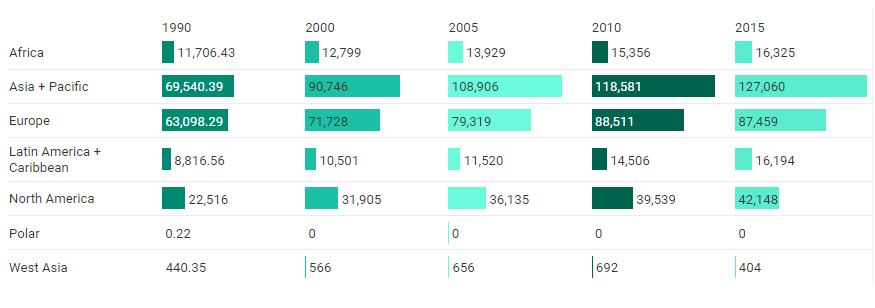
\includegraphics[width=1\linewidth]{Introduction/forestplantation.png}
\caption[Planted Forest Area from 1990 to 2015 in thousand of hectares]{Planted Forest Area from 1990 to 2015 in thousand of hectares. Forest plantation is a forest established by planting and/or seeding in the process of afforestation or reforestation. It consists of introduced species or, in some cases, indigenous species. Forest plantation and natural forests are included in the term forest, a term that refers to land with a tree cover of more than 10 percent and area of more than 0.5 ha. Forests are determined both by the presence of trees and the absence of other predominant land uses. The trees should be able to reach a minimum height of 5 m. Young stands that have not yet reached, but are expected to reach, a crown density of 10m percent and tree height of 5 m are included under forest, as are temporarily unstocked areas. The term includes forests used for purposes of production, protection, multiple use or conservation (i.e. forest in national parks, nature reserves and other protected areas), as well as forest stands on agricultural lands (e.g. windbreaks and shelterbelts of trees with a width of more than 20 m) and rubberwood plantations and cork oak stands. The term specifically excludes stands of trees established primarily for agricultural production, for example fruit tree plantations. It also excludes trees planted in agroforestry systems. Source: \citep{unep_2018}.}
\label{intro-fig:1}
\end{figure}

Tropical deforestation is a relatively modern event that gained momentum in the second half of the 20th century, more precisely, considerable deforestation in the world during 1990-2015 was almost entirely confined to the tropical regions. Figure \ref{intro-fig:2} shows the percentage of forested land in each region. Asia and Latin America had the highest net loss of forest during the period of 1990 to 2015. 

\begin{figure}[H]
\centering
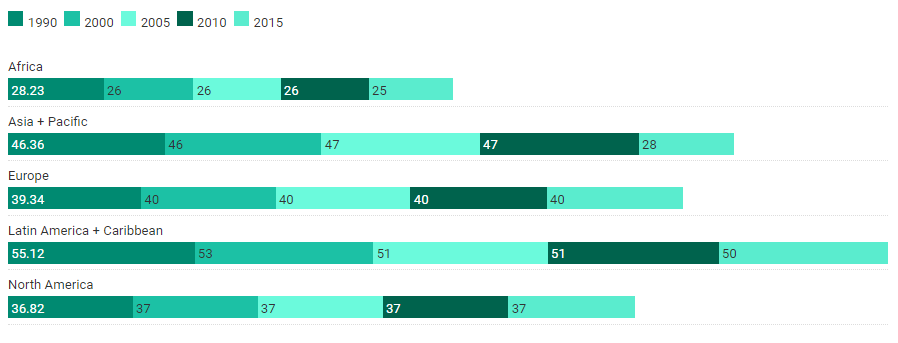
\includegraphics[width=1\linewidth]{Introduction/landcoveredbyforest.png}
\caption[Proportion of land covered by forest from 1990 to 2015 in percentage]{Proportion of land covered by forest from 1990 to 2015 in percentage. Forest: Land spanning more than 0.5 hectares with trees higher than 5 meters and a canopy cover of more than 10 percent, or trees able to reach these thresholds in situ. It does not include land that is predominantly under agricultural or urban land use. Explanatory notes 1. Forest is determined both by the presence of trees and the absence of other predominant land uses. The trees should be able to reach a minimum height of 5 meters in situ. Areas under reforestation that have not yet reached but are expected to reach a canopy cover of 10 percent and a tree height of 5 m are included, as are temporarily unstocked areas, resulting from human intervention or natural causes, which are expected to regenerate. 2. Includes areas with bamboo and palms provided that height and canopy cover criteria are met. 3. Includes forest roads, firebreaks and other small open areas; forest in national parks, nature reserves and other protected areas such as those of specific scientific, historical, cultural or spiritual interest. 4. Includes windbreaks, shelterbelts and corridors of trees with an area of more than 0.5 ha and width of more than 20 m. 5. Includes plantations primarily used for forestry or protection purposes, such as rubberwood plantations and cork oak stands. 6. Excludes tree stands in agricultural production systems, for example in fruit plantations and agroforestry systems. The term also excludes trees in urban parks and gardens. The term is mainly related to FRA 2005 National Reporting Table T1. Source: \citep{unep_2018}.}
\label{intro-fig:2}
\end{figure}

Figure \ref{intro-fig:3} shows that total deforestation across Latin America remains concentrated
in Meso America and South America. This is not surprising, given that this area contains 86\% of the total tropical forest area found in Latin America. Actually, Brazil accounts for 60\% of Latin America’s tropical forests. Thus, the slowdown in deforestation in Brazil is largely responsible for the decline in overall tropical deforestation in Latin America. It is also possible to aggregate information from Figure 1, 2 and 3 in this process, lower middle income and upper middle income accounts for these developing countries from 1990-2000. The decrease in
planted forests means the increase in clearing areas, which corroborates for the scenario.
In other words, many low- and middle-income economies are rapidly changing land use, by converting forests, woodlands and other natural habitat to agriculture and other land-based development activities \citep{BARBIER2}.

\begin{figure}[H]
\centering
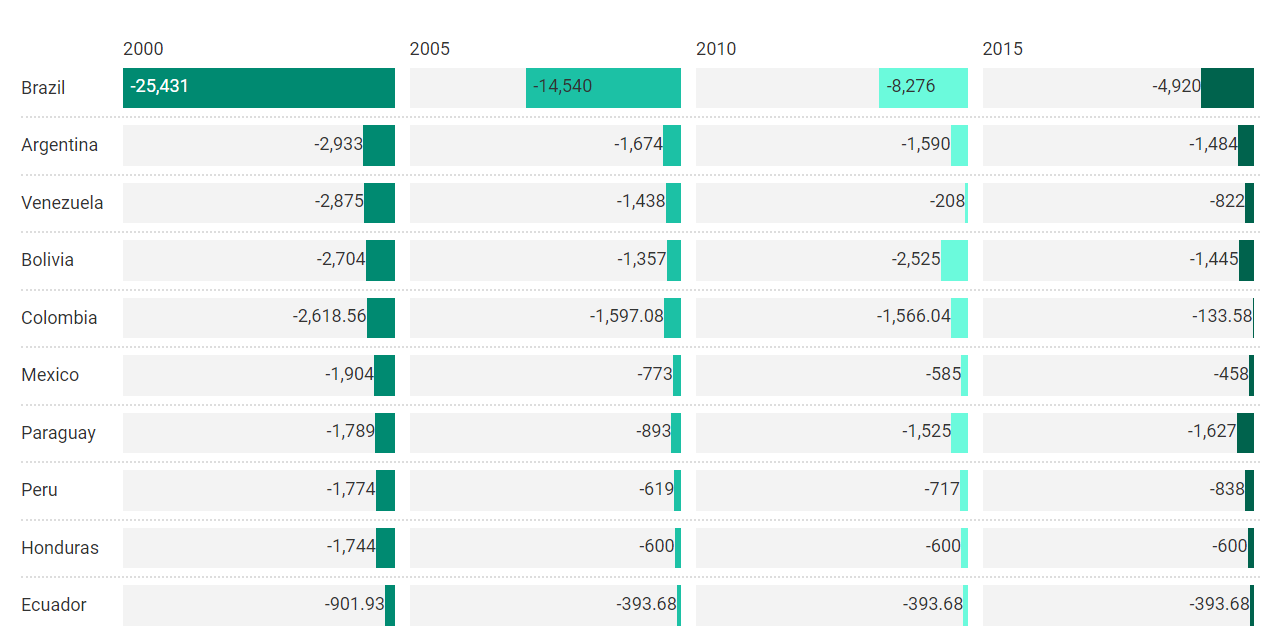
\includegraphics[width=1\linewidth]{Introduction/forestchange_latinamerica.png}
\caption[Forest Average Annual Change from 1990 to 2015 in Thousand Hectares per Year.]{Forest Average Annual Change from 1990 to 2015 in Thousand Hectares per Year. Forest Average Annual Change – Total is the net change in forests and includes expansion of forest plantations and losses and gains in the area of natural forests. Total Forest includes natural forests and forest plantations. The term is used to refer to land with a tree cover of more than 10 percent and area of more than 0.5 ha. Forests are determined both by the presence of trees and the absence of other predominant land uses. The trees should be able to reach a minimum height of 5 m. Young stands that have not yet reached, but are expected to reach, a crown density of 10m percent and tree height of 5 m are included under forest, as are temporarily unstocked areas. The term includes forests used for purposes of production, protection, multiple use or conservation (i.e. forest in national parks, nature reserves and other protected areas), as well as forest stands on agricultural lands (e.g. windbreaks and shelterbelts of trees with a width of more than 20 m) and rubberwood plantations and cork oak stands. The term specifically excludes stands of trees established primarily for agricultural production, for example fruit tree plantations. It also excludes trees planted in agroforestry systems. Source: \citep{unep_2018}.}
\label{intro-fig:3}
\end{figure}

As can be shown, deforestation - specially tropical deforestation - happens in countries where the status of development and welfare of the citizens are crucial factors in determining the extent of the forest loss and the accentuation of deforestation in low income countries is due to poverty, overpopulation and indebtedness. In this sense, the requirement for income and economic growth results in growing demand for agricultural and forest derived products. Facing this, the governments of many developing countries agree that these are the easiest and the most accessible ways of responding to their ever increasing economic pressures \citep{culas11}.

In more recent years, diverse studies are now taking to account the pattern and changes in the rates of environmental transformation in terms of driving forces. More precisely, these studies tries to relates what are the major human causes of land-cover change in different geographical and historical contexts \citep{GEIST}. Proximate and underlying causes of deforestation models are concerned by the fact that some causes are direct in the sense that their occurrence or variation generates more or less deforestation through simple channels and other causes are underlying in the sense that they impact on the sources of deforestation through more complex channels \citep{MOTEL}. 

Specifically, proximate drivers are identified as the hands-on land-management activities that  lead to a land-use conversion or modification of ecosystems \citep{LEEMANS}. \citet*{GEIST2} also define as human activities or immediate actions at the local level, such as agricultural expansion, that originate from intended land use and directly impact forest cover. Underlying driving forces are fundamental social processes that underpin the proximate causes and either operate at the local level or have an indirect impact from the national or global level. In other words, underlying drivers influence the nature and strength of the proximate drivers and include many diverse and often diffuse factors that often operate at more distant different scale levels than the ensuing proximate drivers. In addition, the drivers of deforestation must be defined in their relevant dimensions. This not only means the spatial and temporal dimensions, which are often clearly specified, but also the institutional, legal, organisational, ecological, atmospheric, and other environmental dimensions and their inherent scale levels \citep{LEEMANS}.

Based on several studies\footnote{See references for \citet{culas11, GEIST, GEIST2, LAMBIN2,RICHARDS,RICHARDS2,CARR2,CABRAL,IMORI,DAVALOS,MOLINA,VALENTIM,PFAFF,PFAFF2,PFAFF3,KUIK,COE,SOLER,ZAMBRANO,NEPSTAD,HAMMIG,ARIMA,ARAUJO,VEIGA,BARRETTO,FARELLA,BARNI,CALDAS,COSTA,PATZ}}, it is agreed that the main proximate causes for deforestation in Brazil, the most land converted country in Latin America, are agriculture expansion, cattle ranching, transport infrastructure and settlement expansion. As underlying drivers of tropical deforestation, Brazil deals with the impact of economic growth and the changes on global demand with demographic factors, weak policies and institutional factors. To curb these actions, the implementation of social-political and environmental policies played an essential role.

Broadly, three major barriers to execute effective policies to reduce deforestation are profitability incentives, often in contradiction with forest conservation and sustainable forest management; many proximate and underlying drivers of deforestation lie outside of the forest sector and, limited regulatory and institutional capacity and inadequate resources that constrain the ability of governments to implement forest and sectoral policies related to the forestry sector \citep{TACCONI,GEROLD,FAO3}. 

In this thesis we investigate the effectiveness of the environmental policy implemented in Brazil to curb deforestation considering possible barriers such as, limited regulatory and institutional capacity and inadequate resources that constrain the ability of governments to implement forest policies. The proximate and underlying drivers that lie outside of the forest sector. Environmental factors that contribute to the net forest loss and, profitability incentives, often in contradiction with forest conservation and sustainable forest management. 

%Chapter1
In the first chapter we examine to what extent the Brazil's institutional environmental framework (IEF) has been successful in curbing deforestation by exploring the determinants of Brazilian deforestation for the period 2004-2015. Although previous studies \citep{ARAUJO, OLIVEIRA2,BORGES,NEPSTAD,VALENTIM2,pailler_2018} emphasise the role of institutions in different levels and policy intervention, little has been done concerning the impact of the environmental policy expansion on reducing forest loss and how their effectiveness may be affected by the presence of municipality level institutions for managing environmental policy while controlling for the main driver of deforestation at the present which is market expansion.

This chapter contributes to investigate the impact of both the expansion of the beef, soy and forest product markets and the effectiveness of Brazil's policies to protect the Legal Amazon conditional on the institutional environmental framework (IEF) in place at the time.\footnote{The Legal Amazon is an area that corresponds to 59$\%$ of the Brazilian territory and encompasses all eight states (Acre, Amapá, Amazonas, Mato Grosso, Pará, Rondônia, Roraima and Tocantins) and part of the State of Maranhão (west of the meridian Of 44ºW), totalling more than 5 million km$^{2}$.} We provide a comprehensive analysis at the municipality level where we have detailed information on 562 municipalities where we are able to control for a wide range of possible determinants of deforestation. We employ a panel fixed effects regression model that takes into account environmental policies and prices, and the underlying institutional environmental framework. We expand the analysis by accounting for spatial effects of the model and, we quantify what the level of deforestation may have looked like had Brazil not implemented its current IEF.

Our results suggest that the creation of an institutional environmental framework (IEF) whilst a positive step, was undermined by weak enforcement such that the introduction of environmental laws as an instrument of the National Environmental Policy had little impact on deforestation. However, municipalities who created an environmental office did experience a reduction in the deforestation rate when combined with environmental policies and taking into account an expansion of the market for key commodities. In our spatial analysis we find that the existence of an IEF within municipality has a negative spillover effect on neighbouring municipalities. Our counter-factual simulations show that the monetary benefits of avoiding deforestation and preserving the forest is worth the equivalent to 12 billion tonnes of stored $CO_{2}$.

%Chapter2

In chapter 2, we investigate trends in deforestation in the biome most affected by human occupation over the last three decades in Brazil. Importantly, the Brazilian Cerrado has also been subject to spatially and temporally heterogeneous environmental policies discouraging such deforestation. We document what role such interventionist policies may have played in observed trends in deforestation so it can potentially provide a platform with which to assess future possible scenarios of deforestation in the Cerrado biome and the Amazon forest. We conduct this analysis by using remote sensing data and non-linear models to shape the trends of deforestation and its underlying drivers in the \textit{Cerrado} region in the Brazilian state of Maranhao using the non-linear modelling approach of Generalized Additive Models (GAMs). 

We understand that the state of Maranhão provides a particularly interesting context within which to study trends in deforestation and the possible role of environmental policy. More specifically, Maranhão is divided by an artificial line that separates it in two parts: the Legal Amazon Maranhão and the Cerrado Maranhão. This division, occurring approximately 44$^{\circ}$ west of the meridian, was established in 1953 due to the necessity to plan economic development in the region. This scenario provides a unique natural experiment of deforestation in the Legal Amazon Maranhao (LM) and Cerrado Maranhao (MA) since the former has been subject to fundamentally different environmental policies compared to the latter. More specifically, the tropical forest in the Legal Amazon Maranhao is under a surveillance environmental policy which detects deforestation or fire incidence in the region using satellite data and informs the occurrences to the environmental police so that they can fine or arrest the responsible persons \citep{IBAMAwebsite}. In contrast, this specific environmental policy is not applicable for the other biomes in the Maranhao state. We use this spatial division to determine how deforestation trends may have been different being the Legal Amazon Maranhao and Cerrado Maranhao.

Our use of non-linear modelling for the task at hand derives from the recognition by recent previous research that most ecological and climatic data represent complex relationships and thus that non-linear models, such as GAMs, may be particularly suited to capture confounding effects in trends; see \citep{alkemad_1998,BELL_2015,JOYE_2015,LUSK_2016,SADAT_2016,HALPERIN_2016, SANTOS_2017,TAPIA_2017, LIU_2018,MORENO_2018}. However, a review of the literature shows that such models have only been used sparsely to study deforestation. Here we apply a GAM with a negative binomial distribution and logarithmic link function. We capture deforestation by the construction of monthly time series from remote sensing sources (MODIS), given that high temporal resolution satellite products are particularly suitable to obtain detailed knowledge about the seasonal cycles of vegetation in biomes with strong seasonal contrast, such as the Cerrado biome and Ecotone forest \citep{bayma_sano_2015}. 

We find that for the Legal Maranho region most of the deforestation happened during the rainy season, while in the unprotected Cerrado Maranhão deforestation occurred in the dry season as well. The fact that precipitation and solar incidence also played an important role in deforestation in the rainy season in the Legal Maranhao region, we suggest that cloud cover may have acted as an impediment to infringement detection via satellites, as is conducted by the environmental policy program. We further substantiated this claim by showing that for settlements located in both region but that are not the target of environmental policy deforestation mainly took place during both seasons as well.     

%Chapter3

In our final chapter, we investigate further the findings from  Chapter 2. Apparently, the environmental policy faded in areas of biome transition that coincided with the delimitation of the surveillance policy. We use event history analysis to confirm these findings by considering the heterogeneity within the region because not all sites within ecological tension zone have the same risk of deforestation. The uniqueness of the area proposes a natural experiment of deforestation in the Legal Amazon Maranhão and Cerrado Maranhão since the former has been subject to fundamentally different environmental policies compared to the latter. In our analysis we estimate the probability of a transition between intact forest to disturbed forest, given the risk factors, and conditional on the time elapsed until the occurrence of the transition. We were seeking to answer some questions such as if the probability of deforestation was higher in the region not controlled by a specific environmental policy, what factors may be influencing the risk of the two regions to be deforested, and if changing behaviour undermined the effect of the policy.

Our results show that forests inside the specific surveillance policy area had a lower probability of survival comparing to the area not covered by the environmental policy. Forested pixels close to protected areas,  which include conservation units and indigenous land, had a higher chance of being cleared comparing to forested pixels far from these special zones. The presence of clouds was an active barrier to the legal compliance and, since the studied area has no systematic differences, we can agree on the lack of effectiveness due to cloud barrier.

From this economic and policy analyses of deforestation in Brazil it is possible to derive key policy implications about the potential ways to curb deforestation in the country. We've seen that institutional factors are of great instrument to protect or refrain deforestation in the Legal Amazon however the framework needs to be tightened up in terms of enforcement. We also could follow the past trend of deforestation in two areas of great importance for the Brazilian biome, Amazon and Cerrado. With the trends we could deduce that the deforestation process was shifted to rainy periods and non surveilled areas. The policy implication must to the highest degree be expanded to these ecotonic/transition forests along the Amazon Forest. In addition, monitoring system that could observe deforestation regardless cloud and atmospheric barriers should be considered for the application of the environmental policy such as the satellite Sentinel-2. Finally, since the studied areas are severely influenced by anthropic actions, one step further it would be extending the environmental policy to the Cerrado region. 